\documentclass[12pt,titlepage]{article}
\usepackage[margin=1.25in]{geometry}
\usepackage{graphicx,amsmath}

\makeatletter
\renewcommand*\env@matrix[1][*\c@MaxMatrixCols c]{%
  \hskip -\arraycolsep
  \let\@ifnextchar\new@ifnextchar
  \array{#1}}
\makeatother

%% Variables definition
\newcommand{\vSubject}{Matematika 3}
\newcommand{\vSubtitle}{Eigenvalues and Eigenvector}
\newcommand{\vName}{Dicha Zelianivan Arkana}
\newcommand{\vNIM}{2241720002}
\newcommand{\vClass}{2i}
\newcommand{\vDepartment}{Information Technology}
\newcommand{\vStudyProgram}{D4 Informatics Engineering}

%% [START] Tikz related stuff
\usepackage{tikz}
\usetikzlibrary{svg.path,calc,shapes.geometric,shapes.misc}
\tikzstyle{terminator} = [rectangle, draw, text centered, rounded corners = 1em, minimum height=2em]
\tikzstyle{preparation} = [chamfered rectangle, chamfered rectangle sep=0.75em, draw, text centered, minimum height = 2em]
\tikzstyle{process} = [rectangle, draw, text centered, minimum height=2em]
\tikzstyle{decision} = [diamond, aspect=2, draw, text centered, minimum height=2em]
\tikzstyle{data}=[trapezium, draw, text centered, trapezium left angle=60, trapezium right angle=120, minimum height=2em]
\tikzstyle{connector} = [line width=0.25mm,->]
%% [END] Tikz related stuff

%% [START] Fancy header related stuff
\usepackage{fancyhdr}
\pagestyle{fancy}
\setlength{\headheight}{15pt} % compensate fancyhdr style
\fancyhead{}
\fancyfoot{}
\fancyfoot[L]{\thepage}
\fancyfoot[R]{\textit{\vSubject - \vSubtitle}}
\renewcommand{\footrulewidth}{0.4pt}% default is 0pt, overline for footer
%% [END] Fancy header related stuff

%% [START] Custom tabular command related stuff
\usepackage{tabularx}
\newcommand{\details}[2]{
    #1 & #2  \\
}
%% [END] Custom tabular command related stuff

%% [START] Figure related stuff
\newcommand{\image}[3][1]{
    \begin{figure}[h]
        \centering
        \includegraphics[#1]{#2}
        \caption{#3}
        \label{#3}
    \end{figure}
}
%% [END] Figure related stuff

\begin{document}
\begin{titlepage}
    \centering
    \vfill
    {\bfseries\LARGE
        \vSubject\\
        \vskip0.25cm
        \vSubtitle
    }
    \vfill
    \includegraphics[width=6cm]{images/polinema-logo.png}
    \vfill
    {
        \textbf{Name}\\
        \vName\\
        \vskip0.5cm
        \textbf{NIM}\\
        \vNIM\\
        \vskip0.5cm
        \textbf{Class}\\
        \vClass\\
        \vskip0.5cm
        \textbf{Department}\\
        \vDepartment\\
        \vskip0.5cm
        \textbf{Study Program}\\
        \vStudyProgram
    }
\end{titlepage}

\section{Exercises}
\begin{enumerate}
    \item {
        Find the eigenvalue of A or the value of $\lambda$
        \begin{align*}
            A = \begin{bmatrix}
                 4 & 0 & 1 \\
                -2 & 1 & 0 \\
                -2 & 0 & 1
            \end{bmatrix}
        \end{align*}

        \textbf{Answer}
        \begin{align*}
            Ax &= \lambda x \\
            Ax &= \lambda I x \\
            Ax - \lambda I x &= 0 \\
            (A - \lambda I) x &= 0 \\
            A - \lambda I &= \begin{bmatrix}
                4 & 0 & 1 \\
                -2 & 1 & 0 \\
                -2 & 0 & 1
            \end{bmatrix} - \lambda \begin{bmatrix}
                1 & 0 & 0 \\
                0 & 1 & 0 \\
                0 & 0 & 1
            \end{bmatrix} \\
            &= \begin{bmatrix}
                4 & 0 & 1 \\
                -2 & 1 & 0 \\
                -2 & 0 & 1
            \end{bmatrix} - \begin{bmatrix}
                \lambda & 0 & 0 \\
                0 & \lambda & 0 \\
                0 & 0 & \lambda
            \end{bmatrix} \\
            &= \begin{bmatrix}
                (4 - \lambda) & 0 & 1 \\
                -2 & (1 - \lambda) & 0 \\
                -2 & 0 & (1 - \lambda)
            \end{bmatrix} \\
        \end{align*}
        \begin{align*}
            det(A - \lambda I) &= \begin{bmatrix}[ccc|cc]
                (4 - \lambda) & 0 & 1 & (4 - \lambda) & 0 \\
                -2 & (1 - \lambda) & 0 & -2 & (1 - \lambda) \\
                -2 & 0 & (1 - \lambda) & -2 & 0
            \end{bmatrix} \\
            &= (4 - \lambda)(1 - \lambda)(1 - \lambda) + (0)(0)(-2) + (1)(-2)(0) \\
            &- (1)(1-\lambda)(-2) - (4-\lambda)(0)(0) - (0)(-2)(1-\lambda) \\
            &= (4 - \lambda)(1 - \lambda)^2 + 2(1 - \lambda) \\
            &= (4 - \lambda)(1 - 2\lambda + \lambda^2) + 2(1 - \lambda) \\
            &= 6 - 11 \lambda + 6 \lambda^2 - \lambda^3 \\
            &= -\lambda^3 + 6 \lambda^2 - 11 \lambda + 6 \\
            &= -(\lambda - 1)(\lambda - 2)(\lambda - 3) \\
        \lambda &= 1 \\
        \lambda &= 2 \\
        \lambda &= 3 \\
        \end{align*}
    }
    \pagebreak
    \item {
        Determine the eigenvalue with
        \begin{align*}
            A &= \begin{bmatrix}
                1 & 3 \\
                3 & 1\\
            \end{bmatrix}
            \\
            x &= \begin{bmatrix}
                1 \\
                -1
            \end{bmatrix}
        \end{align*}
        and draw it on a 2-dimensional

        \textbf{Answer}
        \begin{align*}
            Ax &= \lambda x \\
            \begin{bmatrix}
                1 & 3 \\
                3 & 1\\
            \end{bmatrix} \begin{bmatrix}
                1 \\
                -1
            \end{bmatrix} &= \lambda \begin{bmatrix}
                1 \\
                -1
            \end{bmatrix} \\
            \begin{bmatrix}
                1 - 3 \\
                3 - 1
            \end{bmatrix} &= \lambda \begin{bmatrix}
                1 \\
                -1
            \end{bmatrix} \\
            \begin{bmatrix}
                -2 \\
                2
            \end{bmatrix} &= \lambda \begin{bmatrix}
                1 \\
                -1
            \end{bmatrix} \\
            \lambda &= -2 \\
        \end{align*}

        % cartesius coordinate
        \begin{center}
            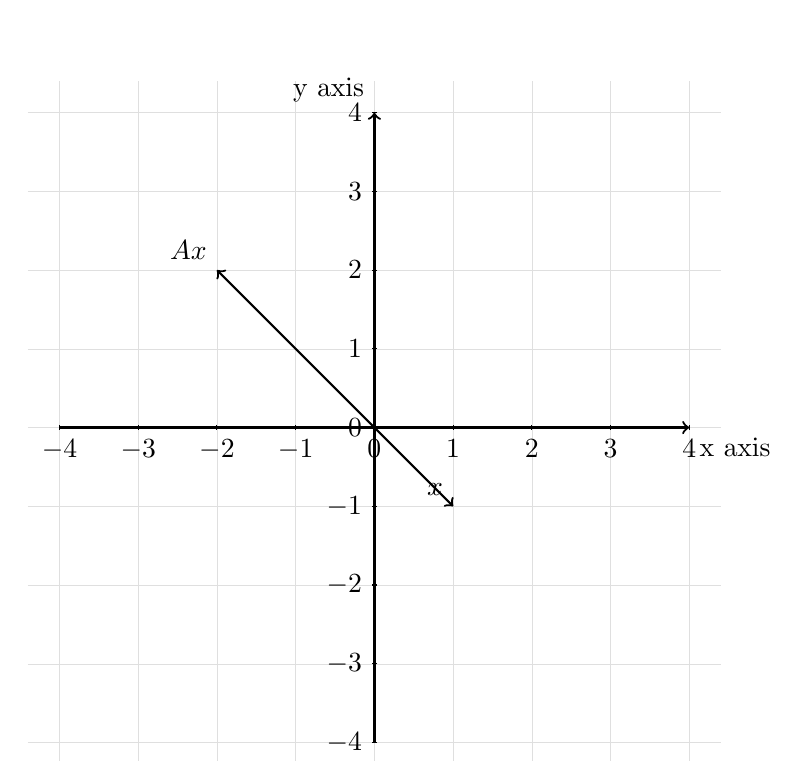
\begin{tikzpicture}
                \draw[step=1cm,gray,very thin,opacity=0.25] (-4.4,-4.4) grid (4.4,4.4);
                \draw[thick,->] (-4,0) -- (4,0) node[anchor=north west] {x axis};
                \draw[thick,->] (0,-4) -- (0,4) node[anchor=south east] {y axis};
                \foreach \x in {-4,-3,-2,-1,0,1,2,3,4}
                    \draw (\x cm,1pt) -- (\x cm,-1pt) node[anchor=north] {$\x$};
                \foreach \y in {-4,-3,-2,-1,0,1,2,3,4}
                    \draw (1pt,\y cm) -- (-1pt,\y cm) node[anchor=east] {$\y$};
                \draw[thick,->] (0,0) -- (1,-1) node[anchor=south east] {$x$};
                \draw[thick,->] (0,0) -- (-2,2) node[anchor=south east] {$Ax$};
            \end{tikzpicture}
        \end{center}
    }
    \pagebreak
    \item {
        Land suitability analysis for maize production in Indonesia using satellite remote sensing and GIS-based multicriteria decision support system\\
        https://link.springer.com/article/10.1007/s10708-019-10091-5
    }s  
\end{enumerate}

\end{document}

